\documentclass[10pt]{article}
\usepackage{icmlko}

\icmlmeta{IP 파운데이션 월드모델}{180}{같은 축이 도메인마다 반대 방향이었다}{노트 179가 ``웹툰 76\%를 버리면 위키 축이 남나''를 남겼다. 버릴 근거가 아니었다 --- 오매칭 몫과 축의 값어치가 안 붙고, 진짜 문제는 부호가 도메인마다 뒤집힌다는 것이었다}

\begin{document}

\twocolumn[
\icmlheader

\begin{abstract}
노트 179가 ``웹툰 정확 매칭의 76\%가 엉뚱한 문서다 --- 그걸 버리면 위키
축이 남나''로 닫았다. 먼저 \textbf{왜 웹툰만 그런지}부터 나왔다.
\textbf{제목 길이다.} 도메인 일곱에서 중앙 제목 길이와 오매칭 몫이
$\rho{=}-0.93$ 으로 붙고, 글자 수로 나누면 \textbf{4자 이하 76.0\% ·
5$\sim$7자 35.5\% · 8$\sim$11자 20.3\% · 26자 이상 6.7\%} 로 단조다(AUC
0.787). 웹툰 제목 중앙이 \textbf{4자}이고 세계애니가 24자다 ---
``해귀''\,``희망''\,``첫정''은 한국어 위키에 그 낱말의 문서가 반드시 있다.
\textbf{이건 부르기 전에 아는 값이다} --- API 를 한 번도 안 부르고 거를 수
있고, 4자 이하만 버리면 오매칭 33.5\%를 잡으면서 옳은 것은 2.3\%만 잃는다.
그다음 \textbf{내 검사기에서 버그 셋}을 찾았다 --- 분류를 받을 때
\texttt{redirects=1} 을 안 붙여 넘겨주기 문서 61건이 분류 0개로 왔고,
음성 분류에 ``낱말''을 넣어 ``긴 낱말''(제목이 긴 정상 문서의 분류)이
라이트 노벨 여덟 건을 걸었다. 고치니 17.9\%가 17.0\%가 된다 ---
\textbf{노트 179의 표는 살아남는다.} 본론. 오매칭이 절반을 넘는 도메인
(웹툰 73\% · 만화 59\%)에서 위키 축을 껐다. \textbf{F18 이 $+$0.0053
($t{=}3.0$)로 오르고 F6 이 $-$0.0031($t{=}-1.9$)로 내린다} --- 형태가
갈린다. 갈랐다. \textbf{부호가 도메인마다 반대다.} 유보에서 옳은 매칭만
보면 세계애니 \textbf{$+$0.35} · 게임 $+$0.21 · 애니 \textbf{$-$0.18}
이고, 학습 구간 일곱 도메인 중 \textbf{넷이 음수}다. 능형은 음수 계수로
그것을 쓰고 트리는 못 쓴다. \textbf{그러니 오매칭 몫은 축을 버릴 근거가
아니다} --- 웹툰은 오매칭 73\%인데 옳은 매칭에서 $\rho{=}-0.32$ 다. 노트
160이 손 축에 만든 부호 파일을 위키 축에도 대 봤다 --- 학습 구간 라벨로만
정해서 $+$0.0018($t{=}0.6$)이다. \textbf{안 갈린다.}
\end{abstract}
]

\begin{figure*}[t]
\centering
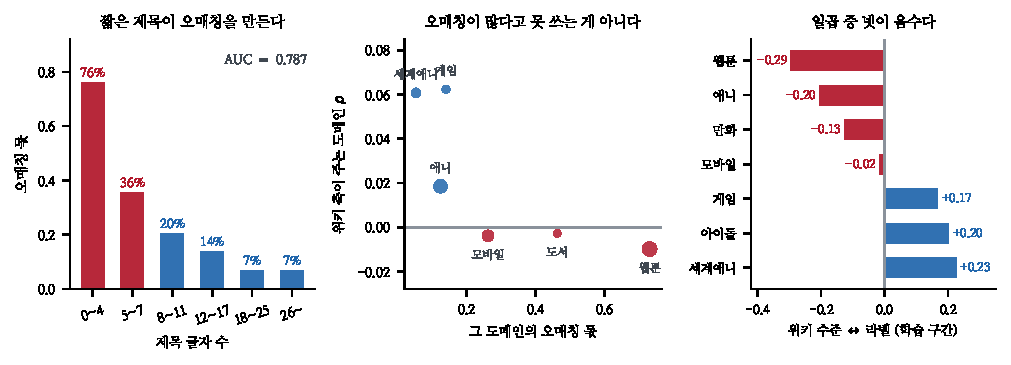
\includegraphics[width=\textwidth]{figs/sign.pdf}
\caption{왼쪽 --- 짧은 제목이 오매칭을 만든다. 가운데 --- 오매칭이 많다고
못 쓰는 게 아니다. 오른쪽 --- 일곱 중 넷이 음수다.}
\end{figure*}

\section{짧은 제목이 오매칭을 만든다}

\begin{table}[t]
\centering\tsize
\caption{제목 글자 수별 오매칭 몫. 2,440건.}
\begin{tabular}{lrr}
\toprule
글자 수 & n & 오매칭 \\
\midrule
\textbf{0$\sim$4} & 192 & \textbf{76.0\%} \\
5$\sim$7 & 197 & 35.5\% \\
8$\sim$11 & 330 & 20.3\% \\
12$\sim$17 & 533 & 13.7\% \\
18$\sim$25 & 491 & 6.7\% \\
\textbf{26$\sim$} & 697 & \textbf{6.7\%} \\
\bottomrule
\end{tabular}
\end{table}

\claimx{\textbf{도메인 사이에서 $\rho{=}-0.93$ 이다.} 웹툰 제목 중앙이
4자(오매칭 73\%)이고 세계애니가 24자(5\%)다. 도메인 \emph{안}에서도
성립한다 --- 만화 AUC 0.849 · 도서 0.725 · 웹툰 0.705.}{까닭이 뻔하다 ---
``해귀''\,``희망''\,``첫정''\,``소방관''은 한국어 위키에 그 낱말의 문서가
반드시 있다. \textbf{짧은 한국어 제목은 거의 다 보통명사다.}}

\begin{table}[t]
\centering\tsize
\caption{글자 수만으로 거르면.}
\begin{tabular}{lrrr}
\toprule
문턱 & 정밀도 & 재현율 & 옳은 것 손실 \\
\midrule
\textbf{$\le$4자} & \textbf{76.0\%} & 33.5\% & \textbf{2.3\%} \\
$\le$7자 & 55.5\% & 49.5\% & 8.6\% \\
$\le$11자 & 39.4\% & 64.9\% & 21.8\% \\
\bottomrule
\end{tabular}
\end{table}

\claimx{\textbf{이건 부르기 전에 아는 값이다.} 분류 규칙은 문서마다 API 를
한 번 더 불러야 했다(1,950번). 글자 수는 레코드만 보면 안다 ---
\textbf{수집을 시작하기 전에 거를 수 있다.}}{4자 문턱이 값이 좋다 ---
오매칭 셋 중 하나를 잡으면서 옳은 것은 마흔 중 하나만 잃는다. 다만
``데미안''\,``이방인''처럼 짧으면서 옳은 것도 있어서 완전한 규칙은 아니다.}

\section{내 검사기에서 버그 셋}

\begin{table}[t]
\centering\tsize
\caption{노트 179의 분류 검사에 있던 잘못.}
\begin{tabular}{ll}
\toprule
\texttt{redirects} & 안 붙여 넘겨주기가 분류 0개로 (61건) \\
``긴 낱말'' & 음성 분류가 정상 문서를 걸음 (8건) \\
낱말 목록 & \texttt{television seasons} 등이 빠짐 \\
\midrule
\textbf{전체 오매칭} & \textbf{17.9\% $\to$ 17.0\%} \\
\bottomrule
\end{tabular}
\end{table}

\claimx{\textbf{노트 179의 표는 살아남는다.} 세 잘못을 다 고쳐도 웹툰
73.1\% · 만화 59.2\% · 세계애니 5.3\% 로 순서와 크기가 그대로다.}{그래도
적어 둘 값이 있다 --- \textbf{검사기를 만들면 검사기도 검사해야 한다.}
``긴 낱말''은 내가 하루 전에 넣은 규칙이 하루 만에 오작동한 것이다.}

\section{반을 넘는 도메인을 껐다}

\begin{table}[t]
\centering\tsize
\caption{웹툰 · 만화의 위키 축을 끄면. 오매칭 몫으로 정했고 판은 안 봤다.}
\begin{tabular}{lrrl}
\toprule
& 판 $\rho$ & 차 & \\
\midrule
현행 (전 도메인) & .4490 & & \\
\textbf{F18} 웹툰·만화 끔 & \textbf{.4542} & $+$.0053 & \textbf{$t{=}3.0$} \\
\midrule
현행 (전 도메인) & .3709 & & \\
\textbf{F6} 웹툰·만화 끔 & .3680 & $-$.0031 & \textbf{$t{=}-1.9$} \\
\bottomrule
\end{tabular}
\end{table}

\claimx{\textbf{두 형태가 반대로 간다.} 트리는 갈리게 오르고 능형은 거의
갈리게 내린다.}{노트 155부터 여덟 번째로 같은 자리다 --- \textbf{판을
올리는 것과 쓸모 있는 것이 형태마다 다르게 답한다.} 이번에는 판정치 자체가
둘로 갈렸다.}

\section{부호가 도메인마다 반대다}

\begin{table}[t]
\centering\tsize
\caption{위키 수준 $\leftrightarrow$ 라벨. 옳은 매칭만.}
\begin{tabular}{lrrrr}
\toprule
& \multicolumn{2}{c}{유보 ($\ge$2025)} & \multicolumn{2}{c}{학습} \\
& n & $\rho$ & n & $\rho$ \\
\midrule
\textbf{세계애니} & 261 & \textbf{$+$.35} & 1294 & $+$.23 \\
게임 & 76 & $+$.21 & 134 & $+$.17 \\
아이돌 & --- & --- & 41 & $+$.20 \\
\midrule
\textbf{애니} & 223 & \textbf{$-$.18} & 459 & $-$.20 \\
\textbf{웹툰} & 18 & --- & 176 & \textbf{$-$.29} \\
만화 & --- & --- & 297 & $-$.13 \\
모바일 & --- & --- & 154 & $-$.02 \\
\bottomrule
\end{tabular}
\end{table}

\claimx{\textbf{일곱 중 넷이 음수다.} 유보에서도 세계애니 $+$0.35 · 게임
$+$0.21 대 애니 $-$0.18 로 부호가 갈린다.}{읽기가 하나 있다 --- 세계애니와
게임은 \emph{그 작품 자신의} 문서에 붙고, 애니 · 웹툰 · 만화는 한국어
위키에서 \emph{원작} 문서에 붙는다. 원작이 유명한 작품은 이미 팬이 있고
새 라벨(즐겨찾기 · 시청)은 신작이 더 크게 먹는다. \textbf{자료로는 못
가른다.}}

\claimx{\textbf{그래서 두 형태가 갈렸다.} 능형은 도메인을 가로질러 계수
하나를 쓰므로 음수 도메인을 끄면 그 계수가 설명하던 것을 잃는다. 트리는
그 부호를 애초에 잘 못 쓰고 있었다.}{\textbf{그리고 오매칭 몫은 축을 버릴
근거가 아니다} --- 웹툰은 오매칭이 73\%인데 옳은 매칭 194건에서
$\rho{=}-0.32$ 다. 노트 179가 보인 대로 \textbf{틀린 값은 이미 죽어 있고
옳은 값은 여전히 산다.}}

\section{부호를 맞춰 붙이면}

\begin{table}[t]
\centering\tsize
\caption{음수 도메인의 위키 축을 뒤집는다. 부호는 2025년 이전 라벨로만.}
\begin{tabular}{lrrl}
\toprule
& 차 & sd & \\
\midrule
F18 배깅 & $+$.0018 & .0026 & $t{=}0.68$ \\
F6 능형 & $+$.0018 & .0030 & $t{=}0.58$ \\
\bottomrule
\end{tabular}
\end{table}

\claimx{\textbf{안 갈린다.} 능형에 $+$0.004$\sim$$+$0.012 를 예측했는데
$+$0.0018 이다. 트리 예측($+$0.000$\sim$$+$0.003)은 맞았다.}{규약은
지켰다 --- 부호를 2025년 이전 행으로만 정했다. 노트 160이 팝업을 뺀 까닭이
``그 결정에 유보 라벨이 필요해서''였고, 여기서는 일곱 도메인 다 학습
표본이 41$\sim$1,294건이라 유보를 안 봐도 정해진다.}

\claimx{\textbf{가드 열둘 전부 통과한다}(\texttt{trendcalwiki} ·
F18 배깅). 분류 검사를 기본으로 켠 판에서 확인했다.}{맨몸 · 귀착 · 시점을
포함해 하나도 안 걸린다.}

\begin{table}[t]
\centering\tsize
\caption{남은 것.}
\begin{tabular}{ll}
\toprule
\textbf{원작 가설} & 음수 도메인이 원작 문서에 붙는지 안 쟀다 \\
글자 수 & 수집 앞단에 문턱을 넣을 것인가 \\
웹툰 유보 & 옳은 매칭이 18건뿐 --- 유보에서 못 잰다 \\
\bottomrule
\end{tabular}
\end{table}

첫 줄이 곧바로 잴 수 있다. ``애니 · 웹툰 · 만화는 원작 문서에 붙는다''는
읽기는 분류로 검정할 수 있다 --- 붙은 문서의 분류가 \texttt{소설} ·
\texttt{라이트 노벨} · \texttt{만화}면 원작이고 \texttt{애니메이션} ·
\texttt{텔레비전} 이면 그 작품 자신이다. \textbf{원작 쪽에서만 부호가
음수면 읽기가 맞고, 둘 다 음수면 틀린다.}

\end{document}
